% Rheological scheme of the cell Hill chain SEE -- (CE || damper || PEE), as in equations.tex (fig:rheo).
% Build: pdflatex hill_rheology.tex && pdftocairo -svg hill_rheology.pdf hill_rheology.svg
\documentclass[tikz,border=4pt]{standalone}
\usetikzlibrary{decorations.pathmorphing,arrows.meta,calc}
\tikzset{
	spring/.style={decorate,decoration={zigzag,amplitude=2.6mm,segment length=2.2mm,
		pre length=3mm,post length=3mm},thick},
	bar/.style={thick},
	ce/.style={draw,thick,fill=gray!15,minimum width=16mm,minimum height=7mm,inner sep=1pt},
	dim/.style={{Latex[length=2mm]}-{Latex[length=2mm]},thin},
	force/.style={-{Latex[length=3mm]},very thick},
}
% dashpot between (#1) and (#2), horizontal, centred
\newcommand{\dashpot}[3][]{%
	\coordinate (dpm) at ($(#2)!0.5!(#3)$);
	\draw[#1] (#2) -- ($(dpm)+(-0.15,0)$);
	\draw[#1] ($(dpm)+(-0.15,-0.22)$) -- ($(dpm)+(-0.15,0.22)$);
	\draw[#1] ($(dpm)+(-0.4,-0.3)$) -- ($(dpm)+(0.3,-0.3)$) -- ($(dpm)+(0.3,0.3)$) -- ($(dpm)+(-0.4,0.3)$);
	\draw[#1] ($(dpm)+(0.3,0)$) -- (#3);
}
\begin{document}
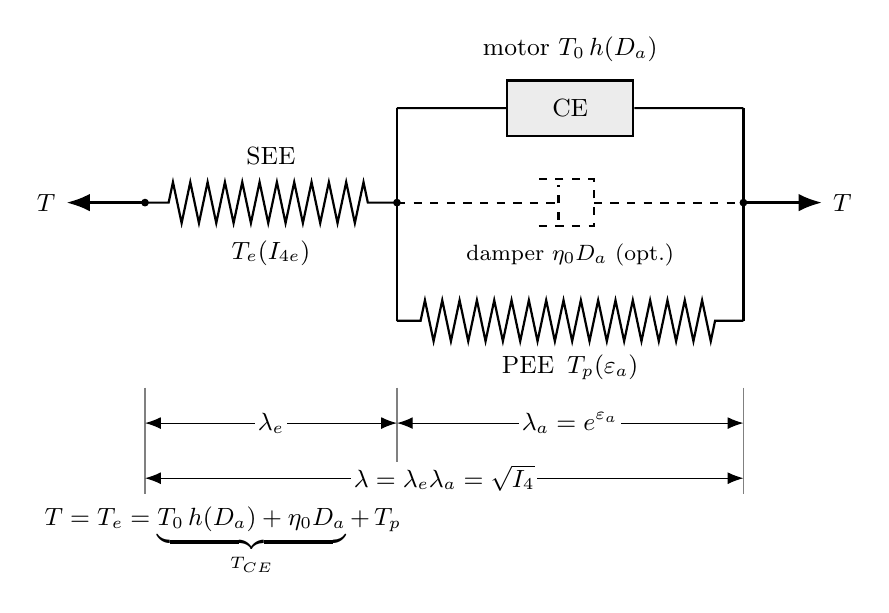
\begin{tikzpicture}[font=\small]
	\coordinate (L) at (0,0);
	\coordinate (A) at (3.2,0);
	\coordinate (B) at (7.6,0);
	% applied tension
	\draw[force] (L) -- ++(-1.0,0) node[left] {$T$};
	\draw[force] (B) -- ++(1.0,0) node[right] {$T$};
	% SEE
	\draw[spring] (L) -- node[above=3.5mm] {SEE} node[below=3.5mm] {$T_e(I_{4e})$} (A);
	% three parallel branches
	\draw[bar] (A) -- ++(0,1.2) coordinate (A1);
	\draw[bar] (A) -- ++(0,-1.5) coordinate (A3);
	\draw[bar] (B) -- ++(0,1.2) coordinate (B1);
	\draw[bar] (B) -- ++(0,-1.5) coordinate (B3);
	% CE (motor)
	\node[ce] (CE) at ($(A1)!0.5!(B1)$) {CE};
	\draw[bar] (A1) -- (CE.west);
	\draw[bar] (CE.east) -- (B1);
	\node[above=1mm] at (CE.north) {motor $T_0\,h(D_a)$};
	% optional damper
	\dashpot[thick,dashed]{A}{B}
	\node[font=\footnotesize,below=1mm] at ($(dpm)+(0,-0.3)$) {damper $\eta_0 D_a$ (opt.)};
	% PEE
	\draw[spring] (A3) -- node[below=3mm] {PEE\enspace $T_p(\varepsilon_a)$} (B3);
	\fill (L) circle (1.4pt) (A) circle (1.4pt) (B) circle (1.4pt);
	% stretches
	\foreach \p in {L,A,B} \draw[thin,gray] ($(\p)+(0,-2.35)$) -- ($(\p)+(0,-3.7)$);
	\draw[dim] ($(L)+(0,-2.8)$) -- node[fill=white,inner sep=1pt] {$\lambda_e$} ($(A)+(0,-2.8)$);
	\draw[dim] ($(A)+(0,-2.8)$) -- node[fill=white,inner sep=1pt] {$\lambda_a = e^{\varepsilon_a}$} ($(B)+(0,-2.8)$);
	\draw[dim] ($(L)+(0,-3.5)$) -- node[fill=white,inner sep=1pt] {$\lambda = \lambda_e\lambda_a = \sqrt{I_4}$} ($(B)+(0,-3.5)$);
	% series equilibrium
	\node[anchor=west] at (-1.4,-4.3) {$T = T_e = \underbrace{T_0\,h(D_a) + \eta_0 D_a}_{T_{CE}} + \,T_p$};
\end{tikzpicture}
\end{document}
